%! TEX program = xelatex
\documentclass[a4paper, 11pt]{report} 

\usepackage{/home/aglaia/Documents/latex-setup/packages/packs}
\usepackage{/home/aglaia/Documents/latex-setup/packages/macros}
\usepackage{/home/aglaia/Documents/latex-setup/packages/mainstyle} 
\usepackage{/home/aglaia/Documents/latex-setup/packages/colors}    
\usepackage{/home/aglaia/Documents/latex-setup/packages/frameboxes} 
\usepackage{/home/aglaia/Documents/latex-setup/packages/title}

\usepackage{bussproofs}
\usetikzlibrary{fit,backgrounds}

\setuniversity{Technische Universität Wien}
\setcoursename{FORSYTE


    \small Formal Methods in Systems Engineering
}
\setcoursebook{slides}
\setauthorname{aglaia norza}
\setauthoremail{norzaglaia@gmail.com}
\setauthorgithub{AglaiaNorza}
\setcoverphoto{cover-meme}

\setcoverwidth{0.6\textwidth}
\setcoverheight{0.6\textwidth}
\setbeforespace{2.5em}
\setafterspace{2.5em}

\begin{document}

\makecustomcover

\tableofcontents
\clearpage

\chapter{Satisfiability in Formal Methods}

\section{The SAT Decision Problem}

\begin{defframe}{The SAT decision problem}{}
    Given a propositional formula in conjunctive normal form, is there a truth assignment to the Boolean variables such that it satisfies all clauses?
\end{defframe}

SAT is an \textit{NP-complete} problem, and it's a very active research area.

\section{Formula transformation}

We have that
\begin{itemize}
    \item every formula can be transformed into an \textbf{equivalent} CNF formula with, in the worst case, an exponential increase in size
    \item every formula can be transformed into an \textbf{equisatisfiable} formula with a \textit{linear} increase in size (by introducing new variables for subformulae)
\end{itemize}

\begin{cframe}{ColorLemma}{Tseitin's transformation}
    \vspace{-1em}
\begin{enumerate}
    \item introduce a fresh boolean variable for every connective
    \item encode each equivalence as a set of clauses
    \item collect all constraints in a big conjunction and enforce the variable representing the entire formula to be true
\end{enumerate}
\end{cframe}

\paragraph{Example.}
Consider the following propositional formula:
\begin{equation*}
\Phi = (a \land (a \lor b)) \lor \neg(a \lor b)
\end{equation*}
First, we break the formula down into an Abstract Syntax Tree (AST) and identify every unique operation, and we then assign a new variable to each (non-atomic) subformula:


\noindent
\begin{minipage}{0.45\textwidth}
\begin{align*}
t_0 &\leftrightarrow (t_1 \lor t_3) \\
t_1 &\leftrightarrow (a \land t_2) \\
t_2 &\leftrightarrow (a \lor b) \\
t_3 &\leftrightarrow \neg t_4 \\
t_4 &\leftrightarrow (a \lor b) 
\end{align*}
\end{minipage}%
\hfill
\begin{minipage}{0.5\textwidth}
\centering
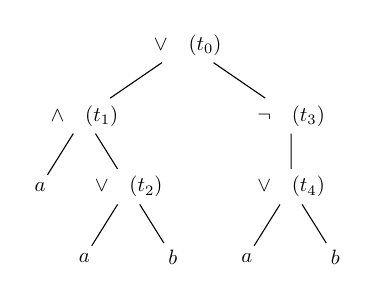
\begin{tikzpicture}[
    scale=0.75, transform shape,
    level distance=1.2cm,
    level 1/.style={sibling distance=3.5cm},
    level 2/.style={sibling distance=1.5cm},
    level 3/.style={sibling distance=1.5cm},
    every node/.style={align=center}
  ]
  
  \node {$\lor \quad (t_0)$}
    child {node {$\land \quad (t_1)$}
      child {node {$a$}}
      child {node {$\lor \quad (t_2)$}
        child {node {$a$}}
        child {node {$b$}}
      }
    }
    child {node {$\neg \quad (t_3)$}
      child {node {$\lor \quad (t_4)$}
        child {node {$a$}}
        child {node {$b$}}
      }
    };
\end{tikzpicture}
\end{minipage}

\vspace{0.5em}
We translate each of these equivalences into standard CNF clauses via:
\begin{itemize}
    \item AND $X \leftrightarrow (Y \land Z)$: \\
    $\equiv (\neg X \lor Y) \land (\neg X \lor Z) \land (X \lor \neg Y \lor \neg Z)$
    
    \item OR $X \leftrightarrow (Y \lor Z)$: \\
    $\equiv (\neg X \lor Y \lor Z) \land (X \lor \neg Y) \land (X \lor \neg Z)$
    
    \item NOT $X \leftrightarrow \neg Y$: \\
    $\equiv (\neg X \lor \neg Y) \land (X \lor Y)$
\end{itemize}

Finally, to assert that the entire formula $\Phi$ is true, we assert the root variable ($t_0$) as a unit clause, and join it with the CNF encodings of all the subformulae:
\begin{align*}
CNF(\Phi) =\; & t_0 \land (t_0 \leftrightarrow (t_1 \lor t_3)) \land (t_1 \leftrightarrow (a \land t_2)) \land (t_2 \leftrightarrow (a \lor b)) \land \\
& (t_3 \leftrightarrow \neg t_4) \land (t_4 \leftrightarrow (a \lor b))
\end{align*}

We get the fully expanded CNF formula:
\begin{align*}
CNF(\Phi) =\; & t_0 \land \\
& (\neg t_0 \lor t_1 \lor t_3) \land (t_0 \lor \neg t_1) \land (t_0 \lor \neg t_3) \land \\
& (\neg t_1 \lor a) \land (\neg t_1 \lor t_2) \land (t_1 \lor \neg a \lor \neg t_2) \land \\
& (\neg t_2 \lor a \lor b) \land (t_2 \lor \neg a) \land (t_2 \lor \neg b) \land \\
& (\neg t_3 \lor \neg t_4) \land (t_3 \lor t_4) \land \\
& (\neg t_4 \lor a \lor b) \land (t_4 \lor \neg a) \land (t_4 \lor \neg b)
\end{align*}

This resulting formula is equisatisfiable to the original $\Phi$.


\begin{cframe}{ColorThm}{Plasted-Greenbaum's transformation}
 Every direction in the Tseitin encoding can be replaced by $\to $ or $\leftarrow $, where the direction of the implication depends on the \textit{polarity} of the formula
        \begin{itemize}
            \item for every occurrence of a subformula $\varphi$, the polarity is $+$ if the number of negations above $\varphi$ in the syntax tree is even, and $-$ otherwise
            \item we add $t_{i} \to $ if the polarity of $t_{i}$ is positive, and $\leftarrow t_{i}$ otherwise
            \item so, every $\to $ and $\leftarrow $ can be replaced by at most two clauses
        \end{itemize}
\end{cframe}

\section{Resolution}
The theory underlying SAT solving is propositional resolution.

\begin{defframe}{Resolution}{}
The resolution rule is:
\vspace{-1em}
\begin{prooftree}
    \AxiomC{$C \cup \{v\}$}
    \AxiomC{$D \cup \{ \neg  v\}$}
    \BinaryInfC{$C \cup D$}
\end{prooftree}
Which tells us that resolving the clause $C \cup \{v\}$ with the clause $D \cup \{\neg v\}$ results in the resolvant clause $D \cup C$.

We also have a \textbf{unit-resolution} rule (or \textbf{BCP}, boolean constraint propagation). This rule can be used on so-called \textit{unit clauses}, clauses with a single literal, which needs to be assigned to $\top$ in a CNF.

\begin{prooftree}
    \AxiomC{$C \cup \{\neg v\}$}
    \AxiomC{$\{v\}$}
    \RightLabel{\quad $\{I, \neg I\} \cap C = \emptyset$}
    \BinaryInfC{$C$}
\end{prooftree}
\begin{gframe}{NB!!}
    This rule is \textit{not refutation-complete}, but  it can be applied in time \textit{linear} to the size of the formula.
\end{gframe}
\end{defframe}

With the unit-resolution rule, we can do \textbf{Unit Propagation}: when a unit resolution produces a unit clause, the unit-resolution step can be repeated with the new clause (until fixpoint).

\begin{cframe}{ColorLemma}{BCP algorithm}
    \begin{itemize}
        \item find a unit clause $I$
        \item remove all the clauses in which $I$ occurs
        \item remove all literals $\neg I$ in clauses
        \item repeat
    \end{itemize}
\end{cframe}

\paragraph{Example}
We want to check the validity of:
$$a \land b \to (a \leftrightarrow b)$$

To check validity, we must check unsatisfiability of the negated formula.
\begin{enumerate}
    \item CNF of negated formula:
    \begin{align*}
    & \neg(a \land b \to (a \leftrightarrow b)) \\
    \equiv\ & a \land b \land \neg(a \leftrightarrow b) \\
    \equiv\ & a \land b \land \neg((\neg a \lor b) \land (a \lor \neg b)) \\
    \equiv\ & a \land b \land (\neg(\neg a \lor b) \lor \neg(a \lor \neg b)) \\
    \equiv\ & a \land b \land ((a \land \neg b) \lor (\neg a \land b)) \\
    \equiv\ & a \land b \land (a \lor \neg a) \land (a \lor b) \land (\neg b \lor \neg a) \land (\neg b \lor b) \\
    \equiv\ & a \land b \land (a \lor b) \land (\neg a \lor \neg b)
    \end{align*}

    \item Unit resolution on $a$ with $(\neg a \lor \neg b)$ \\
    $$a \land b \land (a \lor b) \land (\neg a \lor \neg b) \land (\neg b)$$

    \item Unit propagation:
    $$b \land (\neg b)$$

    \item Unit resolution on $b$ with $(\neg b)$ \\
        $$\text{empty clause}\bot$$
\end{enumerate}
The negation is UNSAT, therefore the original formula is valid.

\section{The DPLL Algorithm}
The DPLL (Davis-Putnam-Logemann-Loveland) algorithm followed the DP (Davis-Putnam) algorithm. Where the first eliminated variables via full resolution, causing an explosion in memory, DPLL branches on variable values, trading memory for execution time (DPLL runs in polynomial space, at the cost of a worst case exponential runtime).


\begin{cframe}{ColorLemma}{DPLL algorithm}
    \begin{itemize}
        \item apply repeated unit resolution and removal of subsumed clauses
            \subitem \textcolor{gray}{at this point, any literals have been removed and the other clauses have been ``cleaned up''}
        \item if $\emptyset \in F$, return UNSAT
        \item if $F = \emptyset$ (no clauses left), return SAT
        \item choose a new variable $x$ (using a decision heuristic), and branch on it:
            \begin{itemize}
                \item add $\{x\}$ and recursively solve
                \item add $\{\neg x\}$ and recursively solve
            \end{itemize}
        \item if one of the branches returns SAT, return SAT
        \item otherwise, return UNSAT
    \end{itemize}

\end{cframe}

There is an optional optimisation that can be added (but that could be too expensive compared to simple BCP):
\begin{gframe}{Pure Literal Rule}
 If a variable appears only with positive polarity (or only negative polarity) throughout $F$:
\begin{itemize}
    \item setting that literal to $\top$ cannot falsify any clause
    \item all clauses containing that pure literal can be eliminated immediately
\end{itemize}
\end{gframe}

\paragraph{Kinds of assignments in DPLL:}
\begin{itemize}
    \item \textbf{Decided ($\bigwedge$):} arbitrary choice/guess when BCP cannot proceed
    \item \textbf{Propagated ($|$):} values logically forced by unit resolution (BCP) until $\bot$ or a stall
\end{itemize}

The main drawback of the DPLL algorithm is its \textbf{blindness to found conflicts}:
\begin{itemize}
    \item  when a conflict ($\bot$) is encountered, DPLL mechanically undoes only the most recent decision and tries the opposite branch, without analyzing which decisions actually caused the conflict (\textit{chronological backtracking})
    \item if a conflict is caused by an independent subset of variables, changing the assignment of an unrelated higher-level variable (like $c$) forces DPLL to rediscover and prove the exact same conflict all over again
    \item DPLL does not remember or record why a dead end was reached; it possesses no memory across distinct branches of the search tree
\end{itemize}

\paragraph{DPLL example: variable choosing}

Let's consider an example:
\[
\mathcal{F} = (\neg b \vee \neg d) \wedge (b \vee \neg d) \wedge (\neg b \vee \neg c) \wedge (b \vee \neg c) \wedge (\neg a \vee c) \wedge (a \vee c \vee d)
\]

Initially, no unit clauses exist, so the solver must decide on an unassigned variable.

The choice of an initial variable can heavily influence the search tree:
\vspace{1em}
\begin{figure}[h!]
\centering
\begin{tikzpicture}[
    decision/.style={circle, draw=blue!70, fill=blue!10, thick, inner sep=2pt, minimum size=6mm},
    prop/.style={rectangle, draw=gray!70, fill=gray!10, rounded corners, inner sep=2pt, minimum size=5mm},
    conflict/.style={rectangle, draw=red!80, fill=red!15, thick, inner sep=2pt, minimum size=5mm},
    edge from parent/.style={draw, thick},
    level 1/.style={sibling distance=38mm, level distance=12mm},
    level 2/.style={sibling distance=20mm, level distance=12mm},
    level 3/.style={sibling distance=16mm, level distance=11mm},
    level 4/.style={level distance=11mm},
    level 5/.style={level distance=11mm}
]

% Tree 1: Decision on 'a'
\node[decision] (root1) {}
    child {
        node[prop] {$c$}
        child {
            node[prop] {$b$}
            child {
                node[conflict] {$\bot$}
            }
        }
        edge from parent node[left] {$a$}
    }
    child {
        node[decision] {}
        child {
            node[prop] {$\neg c$}
            child {
                node[prop] {$\neg d$}
                child {
                    node[conflict] {$\bot$}
                }
            }
            edge from parent node[left] {$b$}
        }
        child {
            node[prop] {$\neg c$}
            child {
                node[prop] {$\neg d$}
                child {
                    node[conflict] {$\bot$}
                }
            }
            edge from parent node[right] {$\neg b$}
        }
        edge from parent node[right] {$\neg a$}
    };

\node[below=2mm of root1, yshift=-5.5cm, align=center] {\textbf{Tree 1:} first decision on $a$\\ (requires 2 decision levels)};

\end{tikzpicture}
\hspace{1.5cm}
\begin{tikzpicture}[
    decision/.style={circle, draw=blue!70, fill=blue!10, thick, inner sep=2pt, minimum size=6mm},
    prop/.style={rectangle, draw=gray!70, fill=gray!10, rounded corners, inner sep=2pt, minimum size=5mm},
    conflict/.style={rectangle, draw=red!80, fill=red!15, thick, inner sep=2pt, minimum size=5mm},
    edge from parent/.style={draw, thick},
    level 1/.style={sibling distance=28mm, level distance=12mm},
    level 2/.style={level distance=12mm},
    level 3/.style={level distance=11mm},
    level 4/.style={level distance=11mm},
    level 5/.style={level distance=11mm}
]

% Tree 2: Decision on 'c'
\node[decision] (root2) {}
    child {
        node[prop] {$b$}
        child {
            node[conflict] {$\bot$}
        }
        edge from parent node[left] {$c$}
    }
    child {
        node[prop] {$\neg a$}
        child {
            node[prop] {$d$}
            child {
                node[prop] {$b$}
                child {
                    node[conflict] {$\bot$}
                }
            }
        }
        edge from parent node[right] {$\neg c$}
    };

\node[below=2mm of root2, yshift=-5.5cm, align=center] {\textbf{Tree 2:} first decision on $c$\\ (no secondary decisions needed)};

\end{tikzpicture}
\caption{DPLL search trees for $\mathcal{F}$. Circles represent decision branch points; rounded rectangles represent literals forced via BCP; and red boxes represent conflict nodes ($\bot$).}
\end{figure}
\vspace{-1em}
\paragraph{DPLL example: blindness to found conflicts}

Consider the formula:
\[
\mathcal{F} = (\neg c \vee a \vee b) \wedge (\neg a \vee \neg b \vee c) \wedge \mathbf{(\neg a \vee \neg b) \wedge (\neg a \vee b) \wedge (a \vee \neg b) \wedge (a \vee b)}
\]
Assume the decision heuristic chooses literals in the order: $\neg c \prec c \prec \neg a \prec a \prec \neg b \prec b$.

\begin{center}
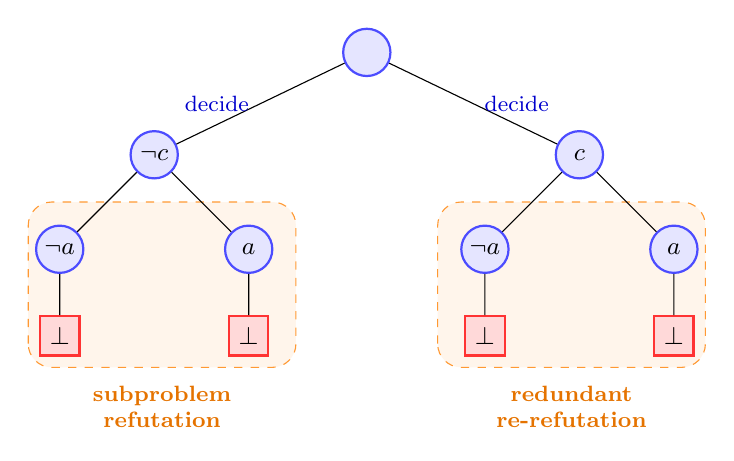
\begin{tikzpicture}[
    level 1/.style={sibling distance=54mm, level distance=13mm},
    level 2/.style={sibling distance=24mm, level distance=12mm},
    level 3/.style={level distance=11mm},
    every node/.style={inner sep=2pt, font=\small},
    dec/.style={circle, draw=blue!70, fill=blue!10, thick, minimum size=6mm},
    conflict/.style={rectangle, draw=red!80, fill=red!15, thick, minimum size=5mm},
    highlight/.style={draw=orange!80, fill=orange!8, dashed, rounded corners=3mm}
]

\draw[highlight] (-4.3, -4.0) rectangle (-0.9, -1.9);
\node[text=orange!90!black, font=\footnotesize, align=center] at (-2.6, -4.5) {\textbf{subproblem}\\\textbf{refutation}};

\draw[highlight] (0.9, -4.0) rectangle (4.3, -1.9);
\node[text=orange!90!black, font=\footnotesize, align=center] at (2.6, -4.5) {\textbf{redundant}\\\textbf{re-refutation}};

\node[dec] (root) {}
    child { node[dec] {$\neg c$}
        child { node[dec] {$\neg a$}
            child { node[conflict] {$\bot$} }
        }
        child { node[dec] {$a$}
            child { node[conflict] {$\bot$} }
        }
        edge from parent node[left=2pt, text=blue!80!black, font=\footnotesize] {decide}
    }
    child { node[dec] {$c$}
        child { node[dec] {$\neg a$}
            child { node[conflict] {$\bot$} }
        }
        child { node[dec] {$a$}
            child { node[conflict] {$\bot$} }
        }
        edge from parent node[right=2pt, text=blue!80!black, font=\footnotesize] {decide}
    };

\end{tikzpicture}
\end{center}

\begin{itemize}
        \item under $\neg c$, splitting on $\neg a$ and $a$ yields contradictions because the subformula over $a, b$ is unconditionally unsatisfiable
        \item chronological backtracking flips $\neg c \to c$.
        \item cnder $c$, DPLL has \emph{no memory} of the previous derivation and blindly duplicates the exact same exploration on $\neg a$ and $a$
\end{itemize}

\section{Clause-Driven Conflict Learning}
Clause-Driven Conflict Learning improves on DPLL by implementing \textbf{backjumping}, a technique that helps to recover from bad decisions by skipping redundant conflicts.

To implement backjumping, one needs to recognise, store and update \textit{which decisions} contributed to conflicts. CDCL solvers achieve this through \textbf{Conflict Analysis} and \textbf{Clause Learning}.

\subsection{Implication Graph}
An \textbf{implication graph} is a labelled DAG $G = (V, E)$ where
\begin{itemize}
    \item $V$ represents the literals of the current partial assignment (\textit{trail})
    \subitem nodes are labelled with their corresponding literal and decision level ($x = v @ d$ where $v \in \{0,1\}$)
    \item $E$ represents the reasons of the assignments
    \subitem edges are labelled with the reason clause used for propagation
\item there is a special node $k$ representing a conflict - it has no outgoing edges, and its incoming edges are:
    $$\{(l, k) | \neg l \in C, C \in F\}$$
    \begin{itemize}
        \item $l$ is a literal node in the implication graph that has been assigned true
        \item $C \in F$ is the clause that caused the conflict (i.e. has been falsified)
        \item $\neg l \in C$ is the qualifying condition for the edge: the negation of $l$ is a component of the clause $C$ ($\neg l$ is false, and this falsification contributes to breaking clause $C$)
        \item $(l,k)$ a directed edge is drawn from the node $l$ to the conflict node $k$, labeled with $C$ to track which clause caused the conflict
    \end{itemize}
\end{itemize}

\begin{gframe}{Example}
Suppose the formula contains the clause $C = (\neg x_1 \lor x_2 \lor \neg x_3)$.

For $C$ to become a conflicting (falsified) clause, the current decision trail must contain the assignments:
\begin{itemize}
    \item $x_1 = \text{true}$ (node $x_1$ exists in the graph)
    \item $x_2 = \text{false}$ (node $\neg x_2$ exists in the graph)
    \item $x_3 = \text{true}$ (node $x_3$ exists in the graph)
\end{itemize}

The nodes responsible for the conflict are $x_1$, $\neg x_2$, and $x_3$. Therefore, the incoming edges to the conflict node $\kappa$ will originate from $x_1$, $\neg x_2$, and $x_3$, representing the assignments that caused $C$ to fail.
\end{gframe}

\paragraph{Implication Graph Example.}
Let the formula $F$ be:
\[ F = C_1 \land C_2 \land C_3 = (\neg a \lor \neg b \lor c) \land (\neg b \lor \neg c) \land (\neg a \lor b) \]

Suppose our first decision is to assign $a$ to true (at decision level 1). This triggers Boolean Constraint Propagation (BCP) as follows:
\begin{enumerate}
    \item $a = 1$ forces $b = 1$ to satisfy $C_3$
    \item $b = 1$ forces $c = 0$ to satisfy $C_2$
    \item now $a = 1$, $b = 1$, and $c = 0$, which falsifies clause $C_1$
\end{enumerate}

This propagation and resulting conflict can be visualized in the implication graph below:
\begin{center}
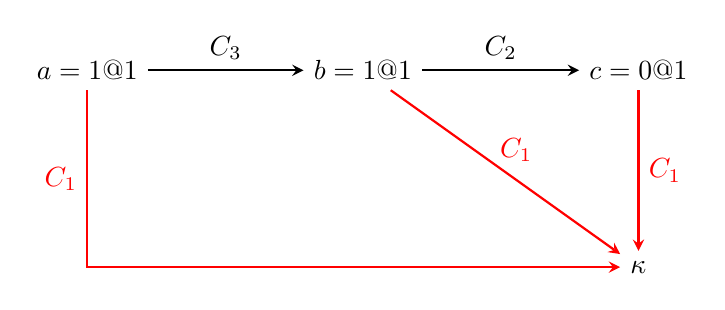
\begin{tikzpicture}[>=stealth, thick]
    \node (a) at (0, 0) {$a = 1 @ 1$};
    \node (b) at (3.5, 0) {$b = 1 @ 1$};
    \node (c) at (7, 0) {$c = 0 @ 1$};
    \node (kappa) at (7, -2.5) {$\kappa$};

    \draw[->] (a) -- node[above] {$C_3$} (b);
    \draw[->] (b) -- node[above] {$C_2$} (c);

    \draw[->, red] (a) |- node[near start, left] {$C_1$} (6.7, -2.5) -- (kappa); 
    \draw[->, red] (b) -- node[above right, xshift=-0.2cm] {$C_1$} (kappa);
    \draw[->, red] (c) -- node[right] {$C_1$} (kappa);
\end{tikzpicture}
\end{center}
\vspace{1em}

\begin{gframe}{Simple implementation details}
In modern CDCL solvers, the implication graph is not stored as an explicit graph data structure. Instead, it is implicitly maintained via the assignment trail (stack of currently assigned variables).

For each assigned variable, we store a tuple \texttt{(Value, Decision Level, Reason Pointer)}:
\begin{itemize}
    \item \textbf{reason pointer (antecedent):} pointer to the clause that forced this assignment
    \subitem storing this pointer allows the solver to instantly trace backward from a conflict to compute a learned clause via resolution, without re-scanning the clause database
    \item \textbf{decision variables:} variables chosen by the decision heuristic (guesses) are not forced by any clause. Their reason pointer is set to \texttt{null} (so,during conflict analysis, a \texttt{null} pointer signifies a root node in the implication graph)
\end{itemize}
\end{gframe}

\subsection{Clause Learning}



\chapter{Algebraic Reasoning}
\chapter{Program Analysis}
\chapter{Model Checking Approaches}


\end{document}
